%\documentclass{article}
\documentclass[]{article}
\usepackage{bm}
\usepackage{amsmath}
\usepackage{amsfonts}
\usepackage{natbib}
\usepackage{graphicx}
\usepackage{placeins}
\usepackage{caption}
\usepackage{subcaption}
\bibliographystyle{unsrtnat}


\begin{document}

\section{Update - February 10th 2021}	
	
	
\subsection{Sample size and speed of simulation}

In the following we test the speed of the code for solving and running the recession scenario. We assume that there is one discount factor common to all agents.

The following table shows the time needed to run the code, that i) solves the model without AD effects, ii) solves the model with AD effects and iii) simulates the considered scenario with and without AD effects.\footnote{40 simulations are performerd here, i.e. recessions that last 1 to 20q, with and without AD effects.} The second point requires solving the model several times repeadetly with macroeconmic beliefs of agents being updated in each iteration. For this reason, this step is by far the most time-intensive. When solving the model with AD effects, the algorithm is terminated when the change in beliefs from one to the next iteration falls below a certain tolerance. The second and third row of the table compare two different levels of that tolerance.\footnote{The change is measured as the Euclidean norm of the difference in slopes and intercepts of the linear function on the consumption ratio, which agents use to predict future income.} Note, that while solving with more agents is somewhat slower, it actually helps the algorithm to find the AD solution with fewer iterations. Simulating the larger number of agents is much slower, however.

\begin{center}
	\begin{tabular}{||c| c |c||} 
		\hline
		  & Sample 50k & Sample 200k \\ [0.5ex] 
		\hline\hline
		Solving without AD &  1 min & 1 min 20 sec  \\ \hline
		Solving with AD (tol: 1E-3) &  10 min ( 10 iter.)  & 12 min (7 iter.)  \\ \hline
		Solving with AD (tol: 1E-4) &  22 min ( 20 iter.)  & 16 min (10 iter.)  \\ \hline
		Simulation & 2 min 20 sec  & 16 min \\ [1ex] 
		\hline
	\end{tabular}
\end{center}

Figure \ref{fig:CRatio} plots $CR_t$ on  $CR_{t-1}$ where $CR_t$ is the ratio of simulated consumption to the baseline consumption in period $t$. The assumption behind our numerical algorithm to solve the model under AD effects is that individuals are able to predict the future consumption ratio, and thus their expected income (taking into account aggregate demand effects), based on a linear function of today's consumption ratio. If that assumption is correct, it should hold, that $CR_t = i + s (CR_{t-1} - 1 )$. Hence, we should see a line with a constant gradient. As seen in the figure, this only holds approximately. A higher sample size somewhat improves the picture, a lower tolerance value for the convergence of macro beliefs does not.

\begin{figure}
	\centering
	\begin{subfigure}[b]{0.45\textwidth}
		\centering
		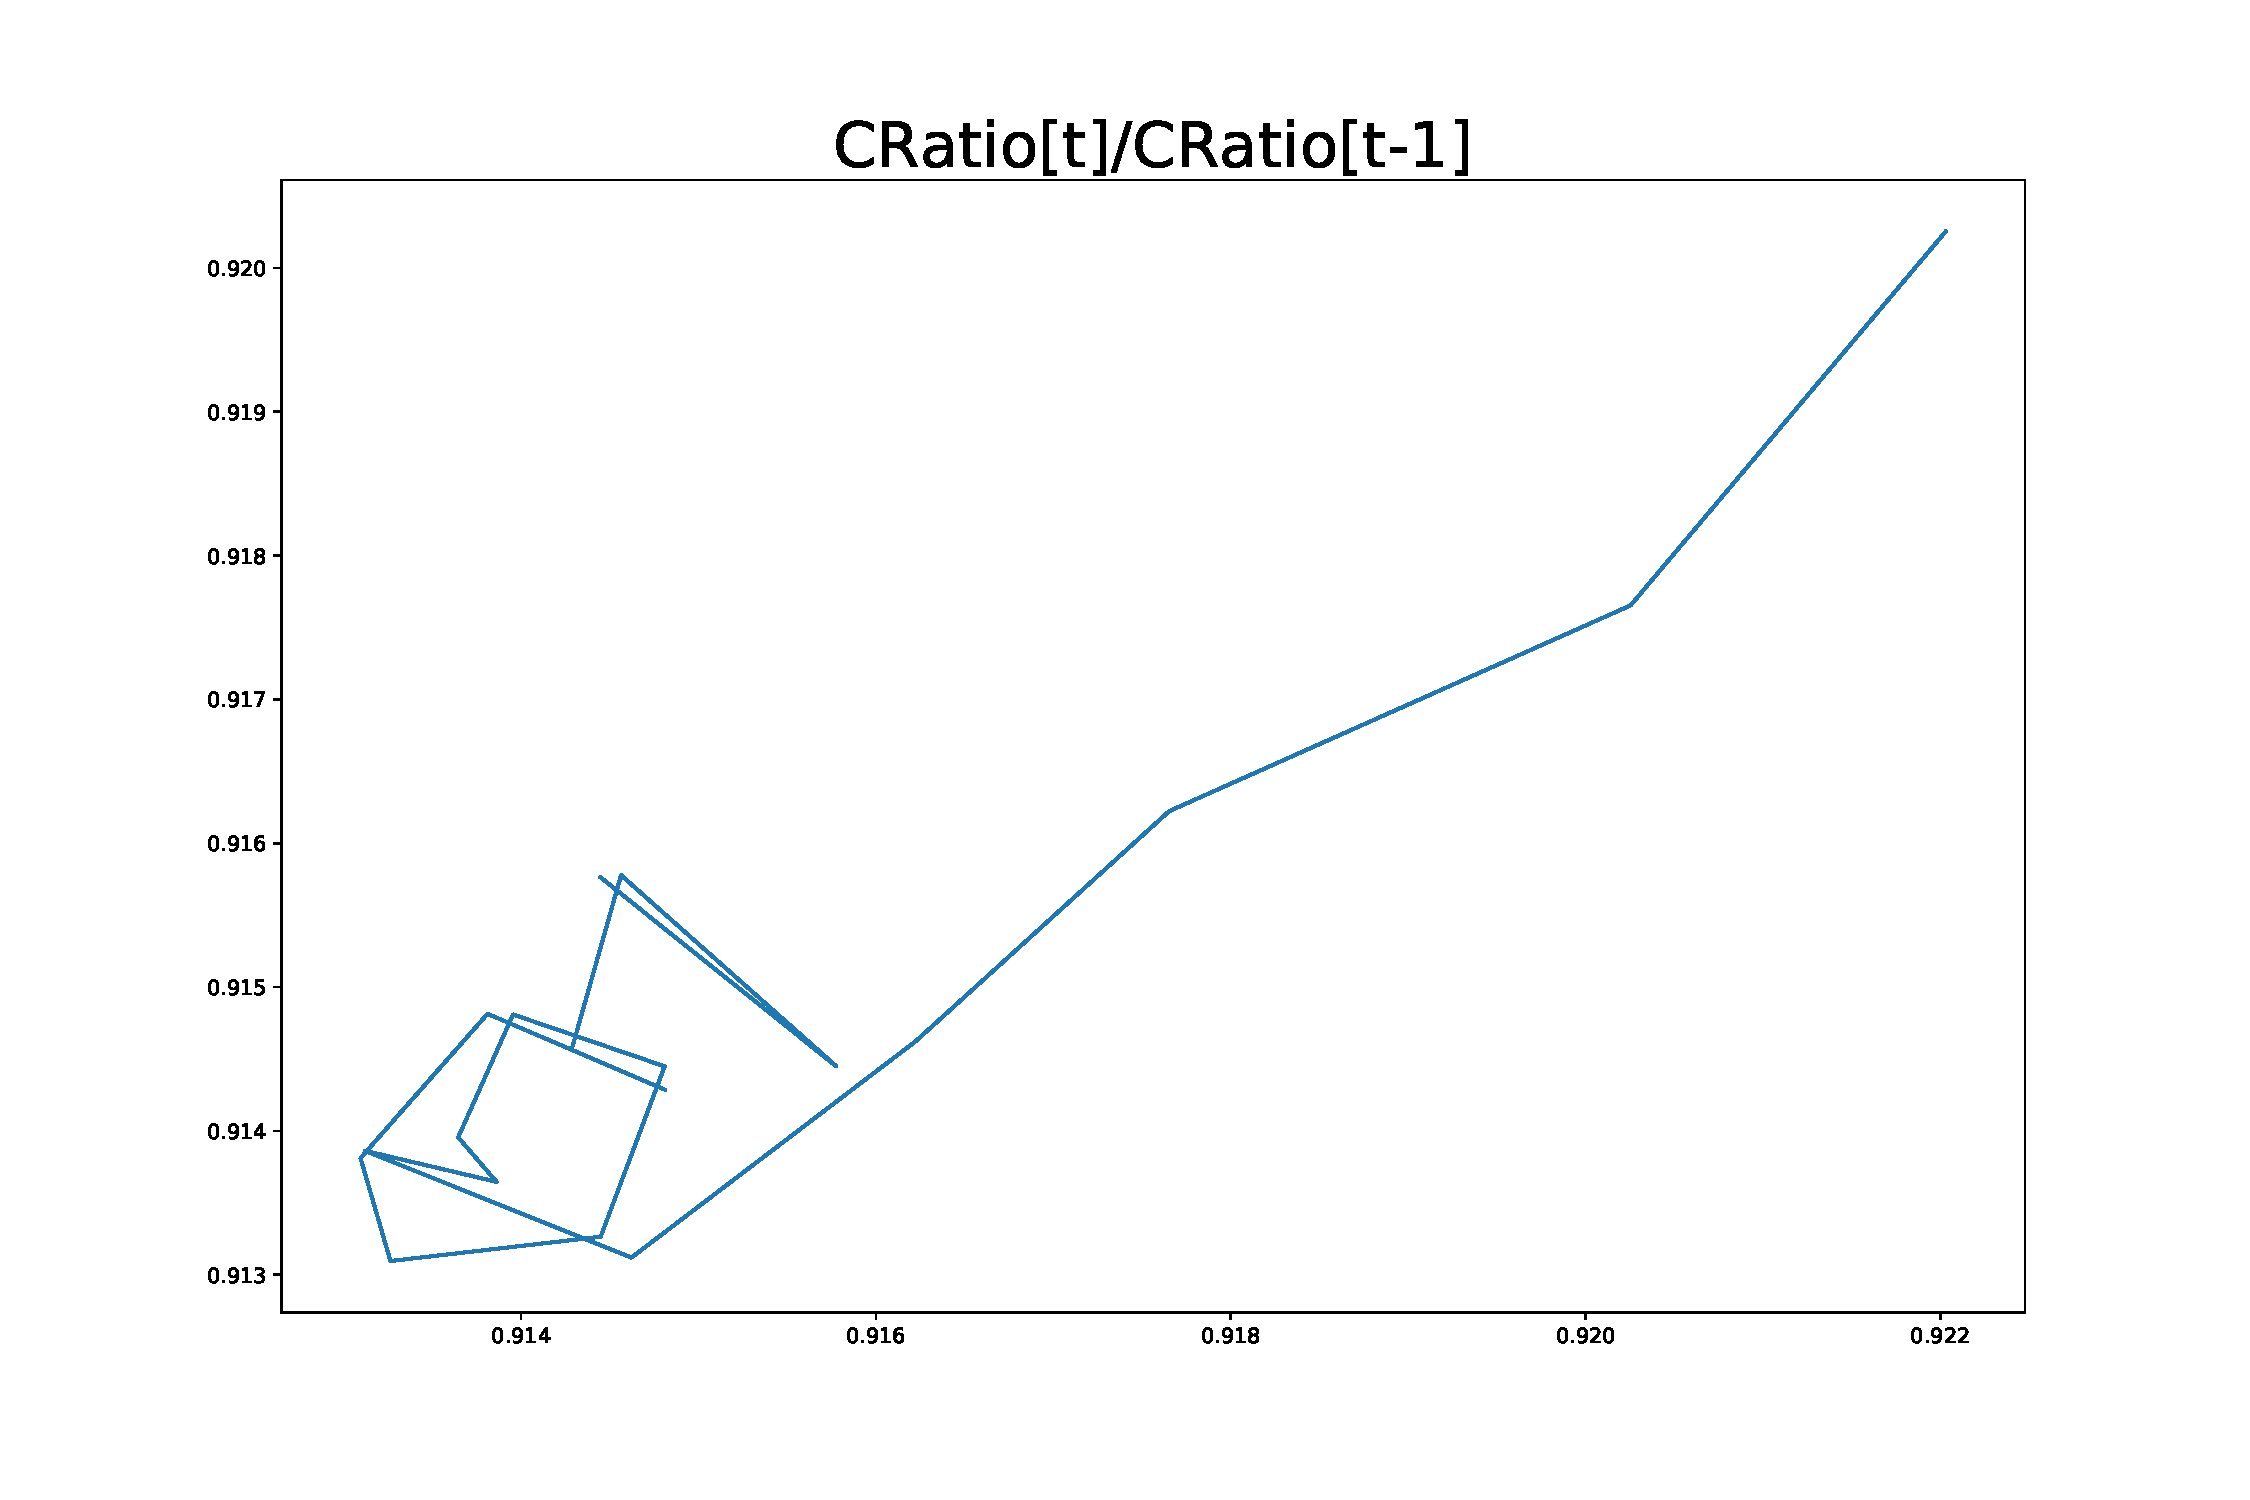
\includegraphics[width=1.2\textwidth]{../50kSample_BaseCal/CRatio.pdf}
		\caption{Sample 50k, tol = 1E-3}
		\label{fig:Cratio-50k-Baseline}
	\end{subfigure}
	\hfill
	\begin{subfigure}[b]{0.45\textwidth}
		\centering
		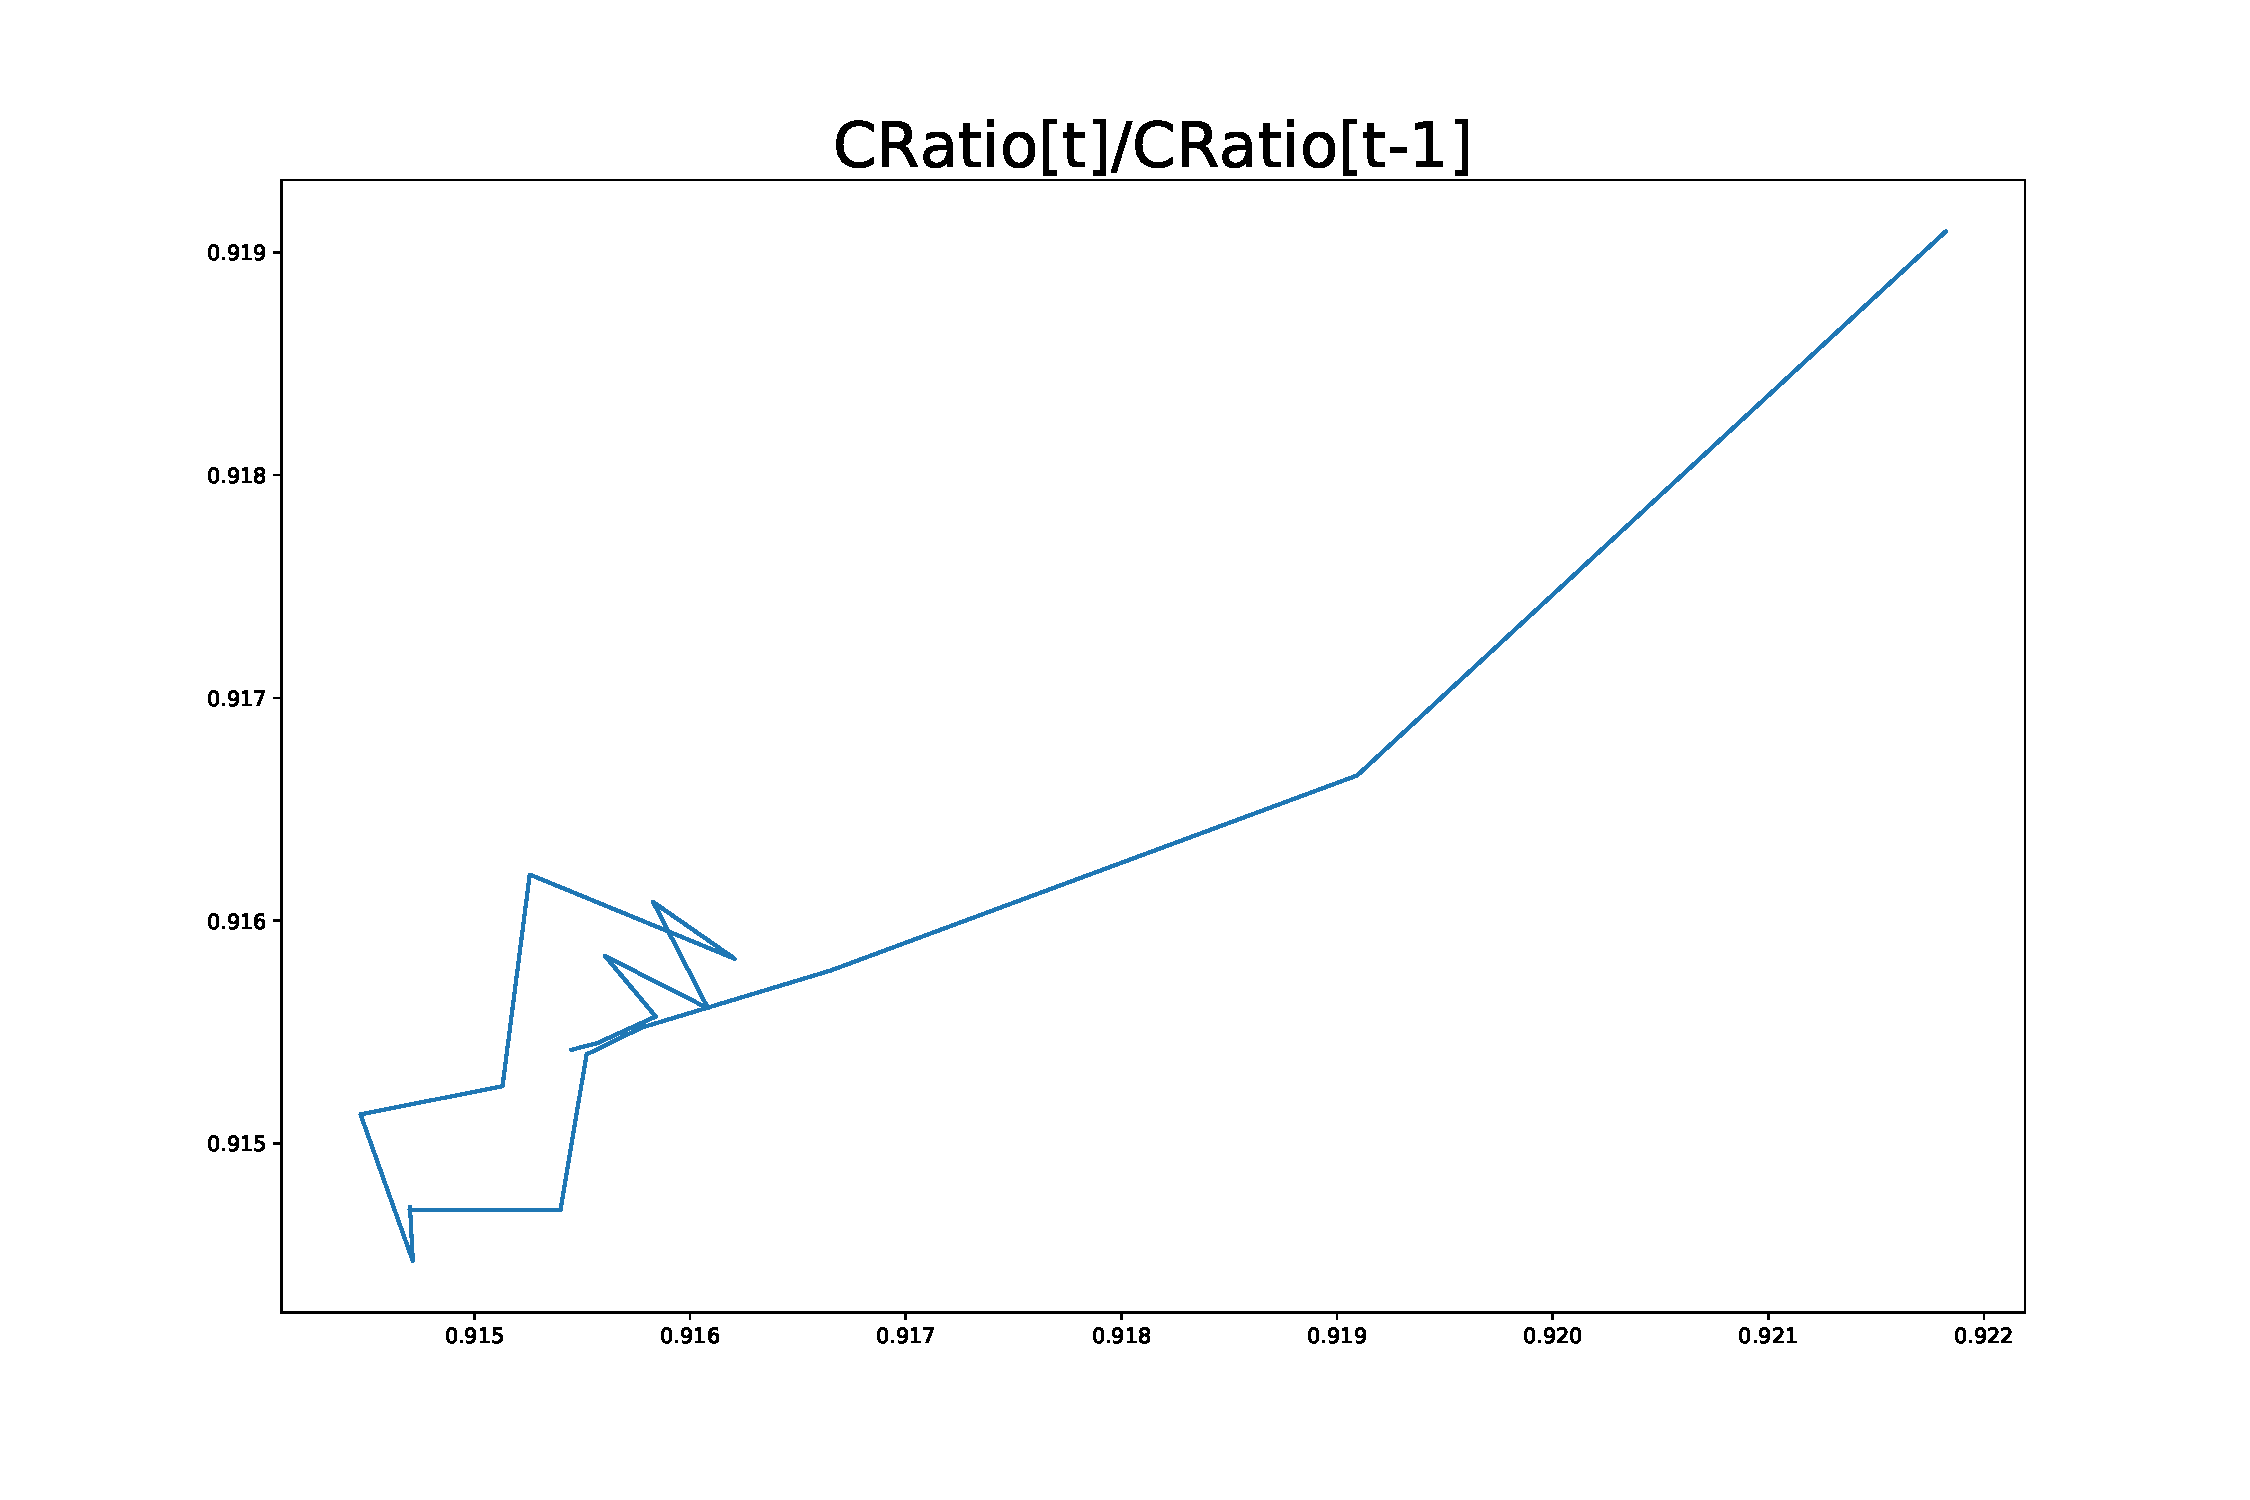
\includegraphics[width=1.2\textwidth]{../200kSample_BaseCal/CRatio.pdf}
		\caption{Sample 200k, tol = 1E-3}
		\label{fig:Cratio-200k-Baseline}
	\end{subfigure}\\
	\begin{subfigure}[b]{0.45\textwidth}
		\centering
		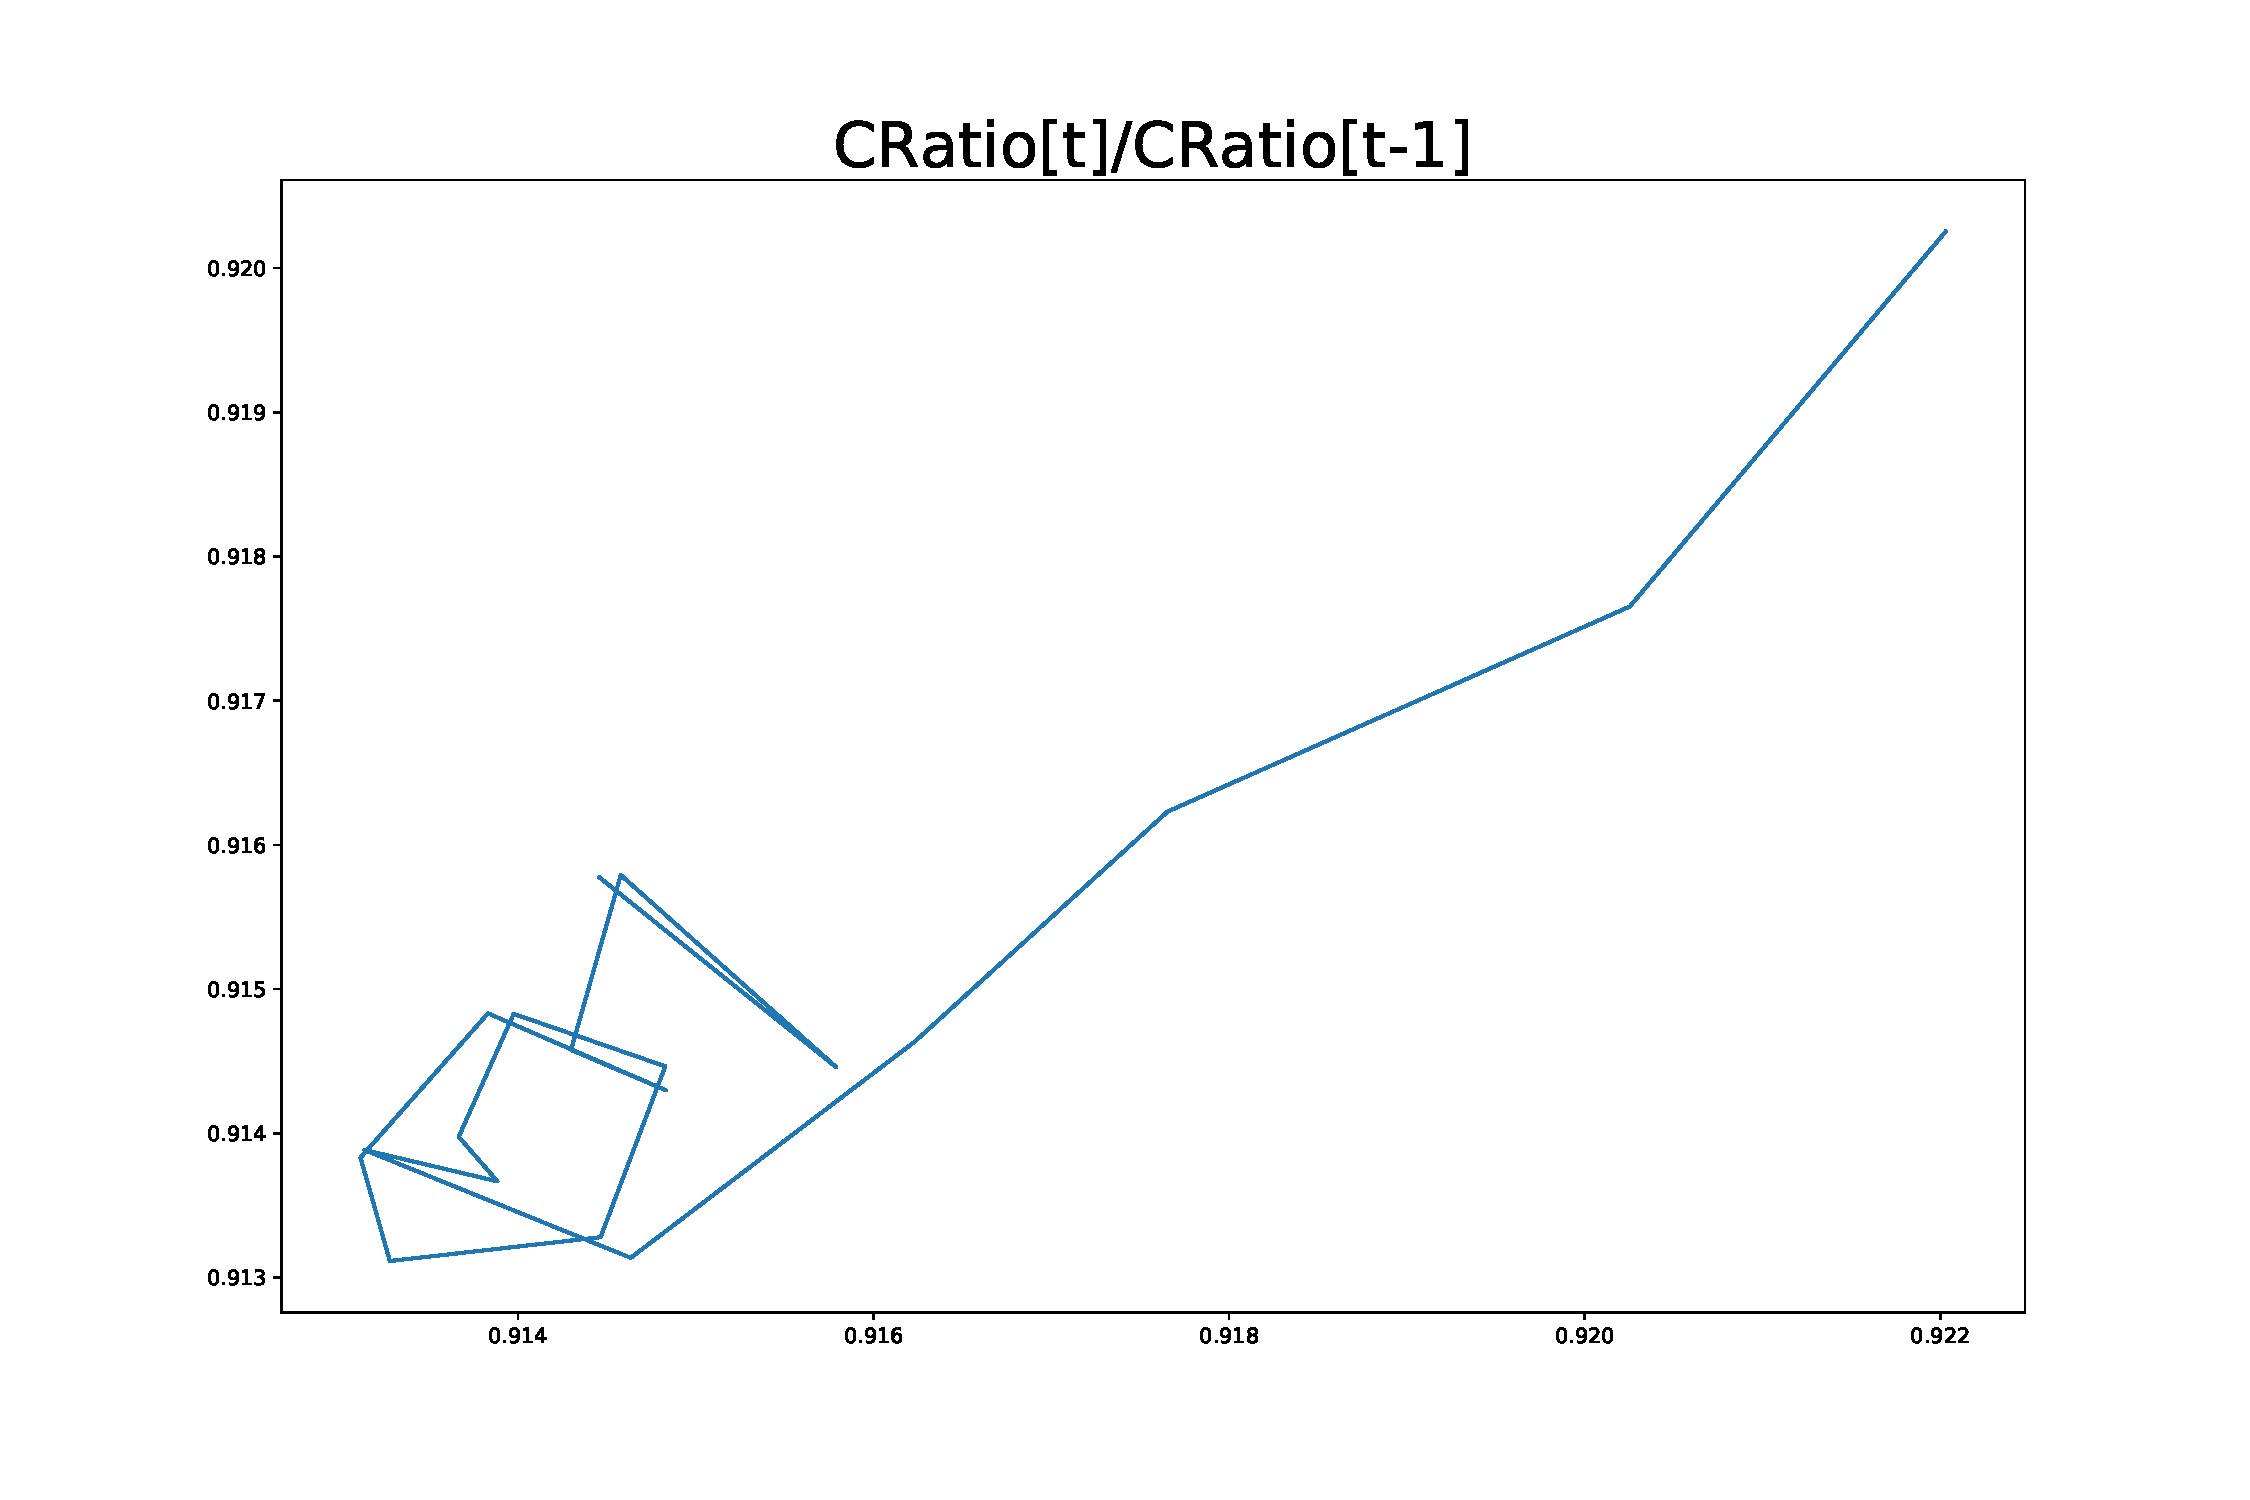
\includegraphics[width=1.2\textwidth]{../50kSample_BaseCal_TolE-4/CRatio.pdf}
		\caption{Sample 50k, tol = 1E-4}
		\label{fig:Cratio-50k}
	\end{subfigure}
	\hfill
	\begin{subfigure}[b]{0.45\textwidth}
		\centering
		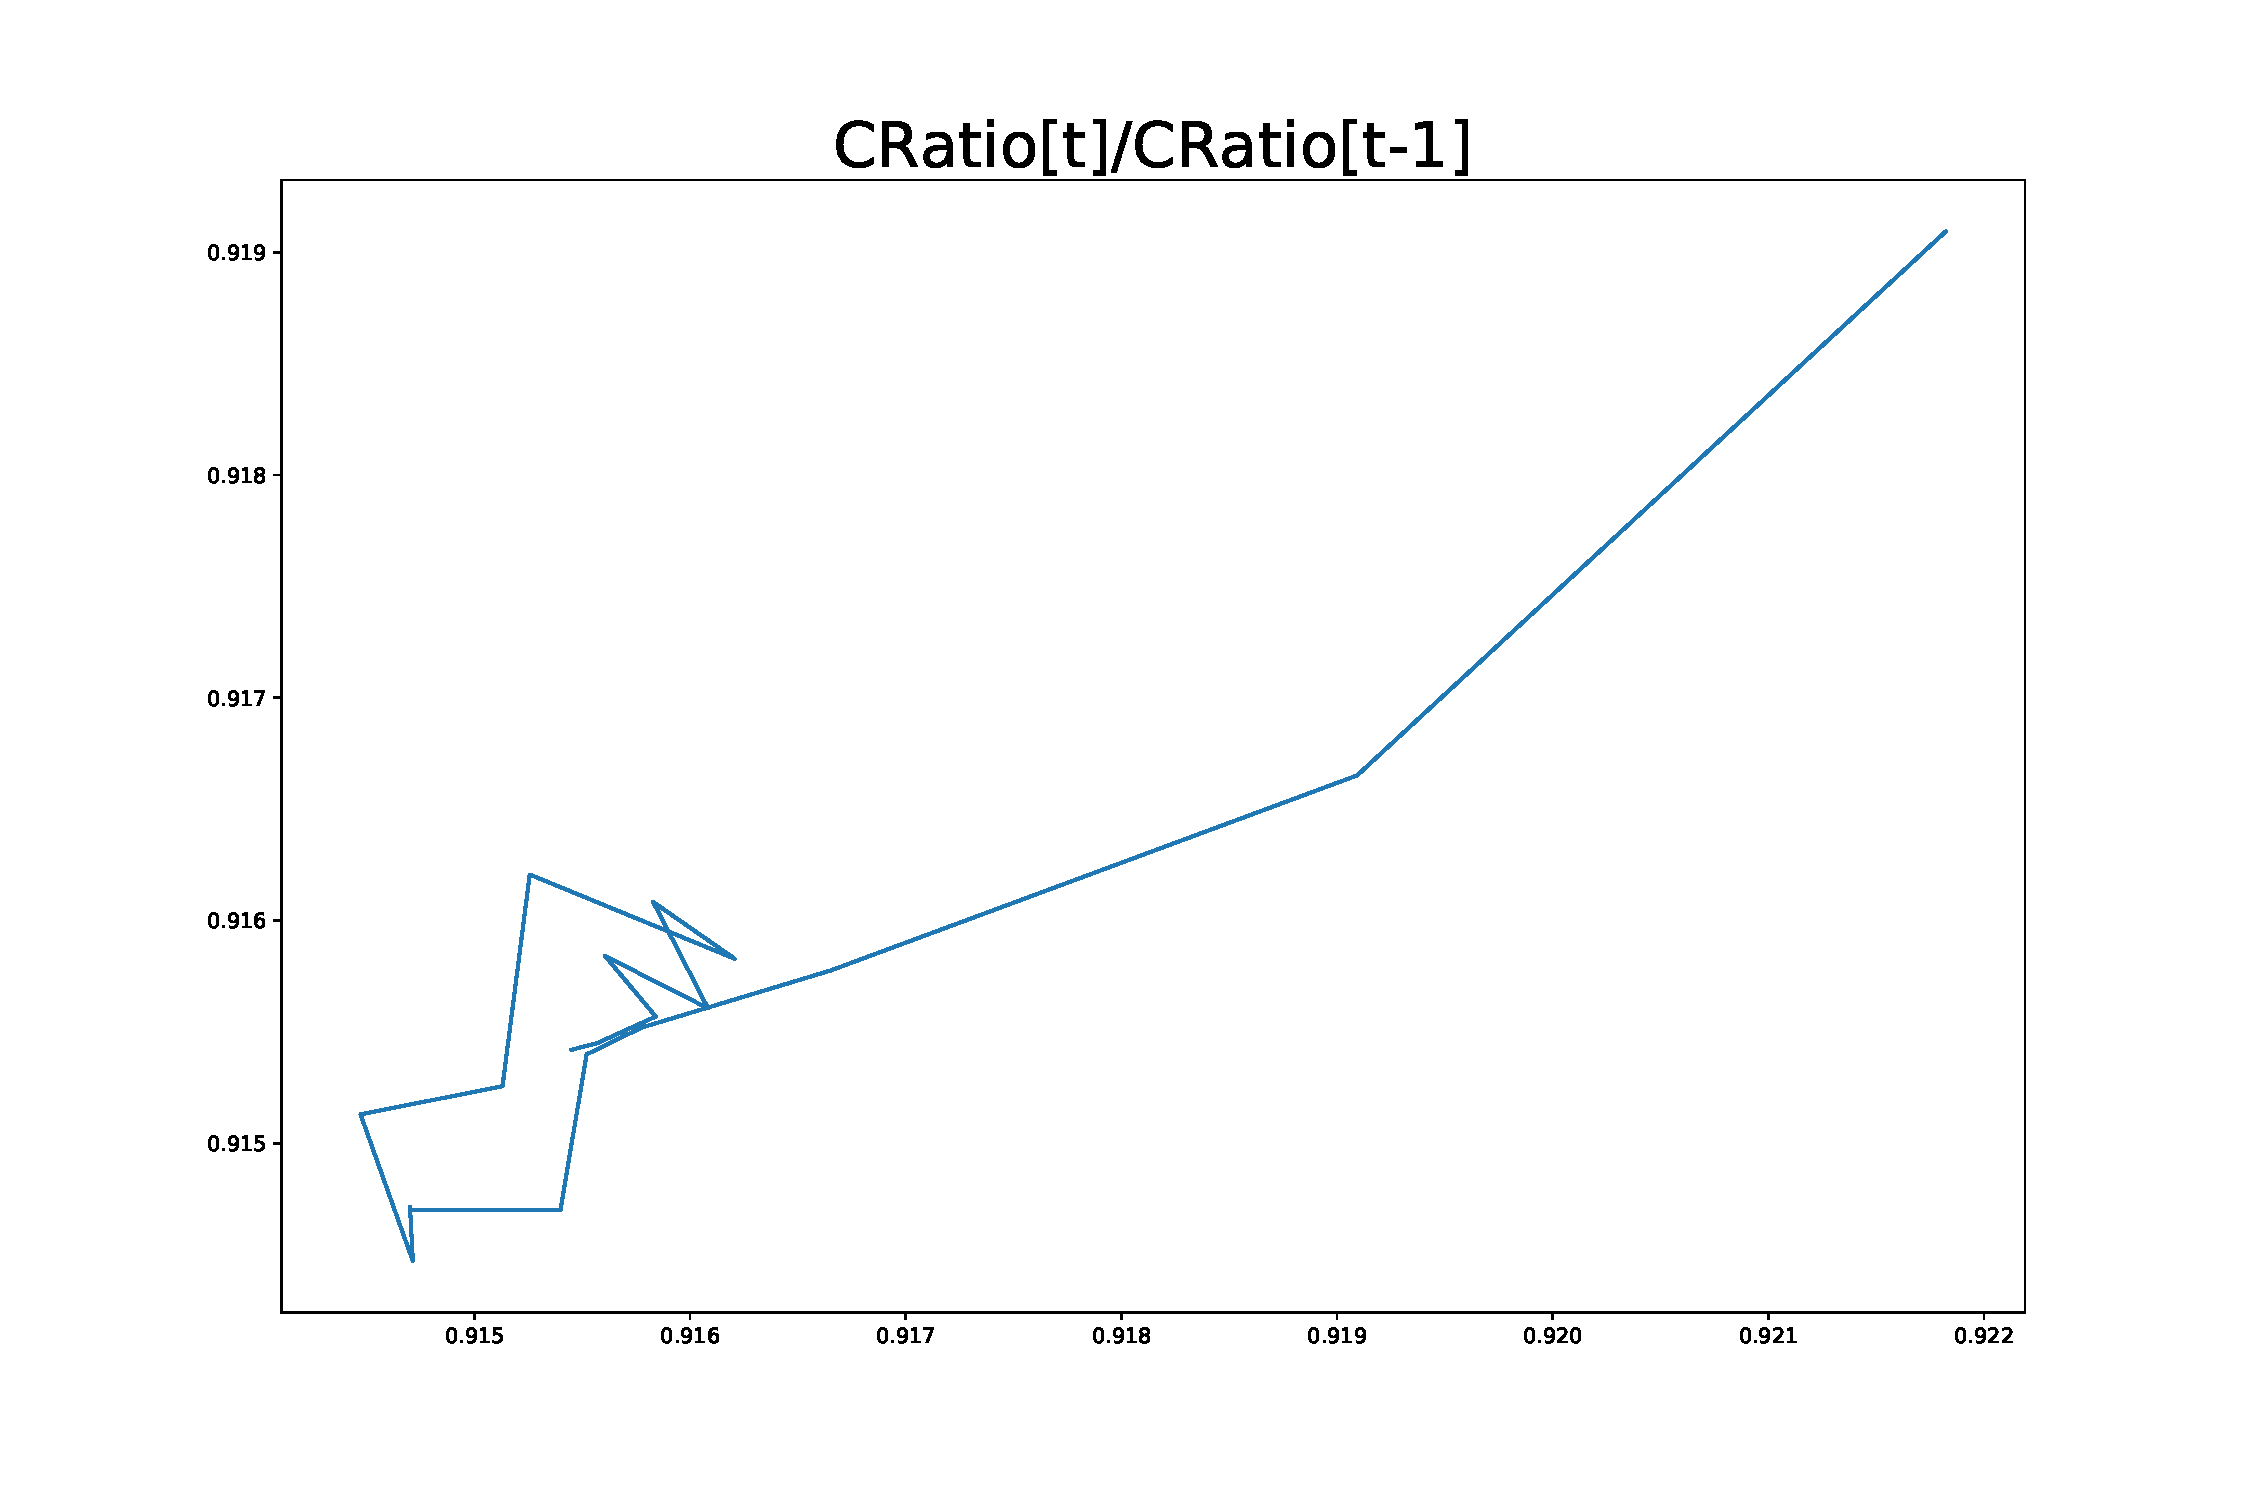
\includegraphics[width=1.2\textwidth]{../200kSample_BaseCal_TolE-4/CRatio.pdf}
		\caption{Sample 200k, tol = 1E-4}
		\label{fig:Cratio-200k}
	\end{subfigure}
	\caption{Plotting $CR_t$ (y-axis) on $CR_{t-1}$ (x-axis). (subfigure's title misleading, please ignore)}
	\label{fig:CRatio}
\end{figure}


\newpage
\section{Update - January 13th 2021}
\begin{itemize}
	\item Last call: impact of a payroll tax cut / extension of unemployment benefits on consumption; there were no aggregate demand effects
	\item Edmund created code to capture AD effects: Current consumption affects TFP: $TFP_t = \left(\frac{C_t}{C_{ss}}\right)^\alpha$ where $\alpha = 0.4$.
	\item What is working so far: AD effects for payroll tax cut experiment, for recession and for payroll tax cut during recession
	\item What is not working yet: AD effects for unemployment benefits extension
\end{itemize}

\section{Stimulus Experiments}

Parametrization
\begin{itemize}
	\item Update probabiltity = 1 (have not tried sticky information yet)
	\item 7 discount factor groups: Beta = 0.986 (center), Nabla = 0.0183 (spread) as estimated on Norwegian Data
	\item Splurge = 0.32 as estimated on Norwegian Data
	\item Simulation of these results takes about 4 h (50k Agents, T-sim = 400)
\end{itemize}	

\subsection{Recession}

\begin{itemize}
	\item We consider a recession with an expected length of 6 quarters, see Figure \ref{fig:recession}
	\item In a recession the unemployment rate increases to 10 \% and lasts on average 4 quarters (as opposed to 5\% / 1.5 q in normal times)
	\item The recession depresses aggregate income due to loss of labor income, only partly compensated by unemployment benefits (lasting 2 q, replacing 30 \% of income)
	\item Consumption falls as income is lower.
	\item The recession is deeper when productivity depends on aggregate demand.
\end{itemize}


\begin{figure} 
	\begin{centering}
		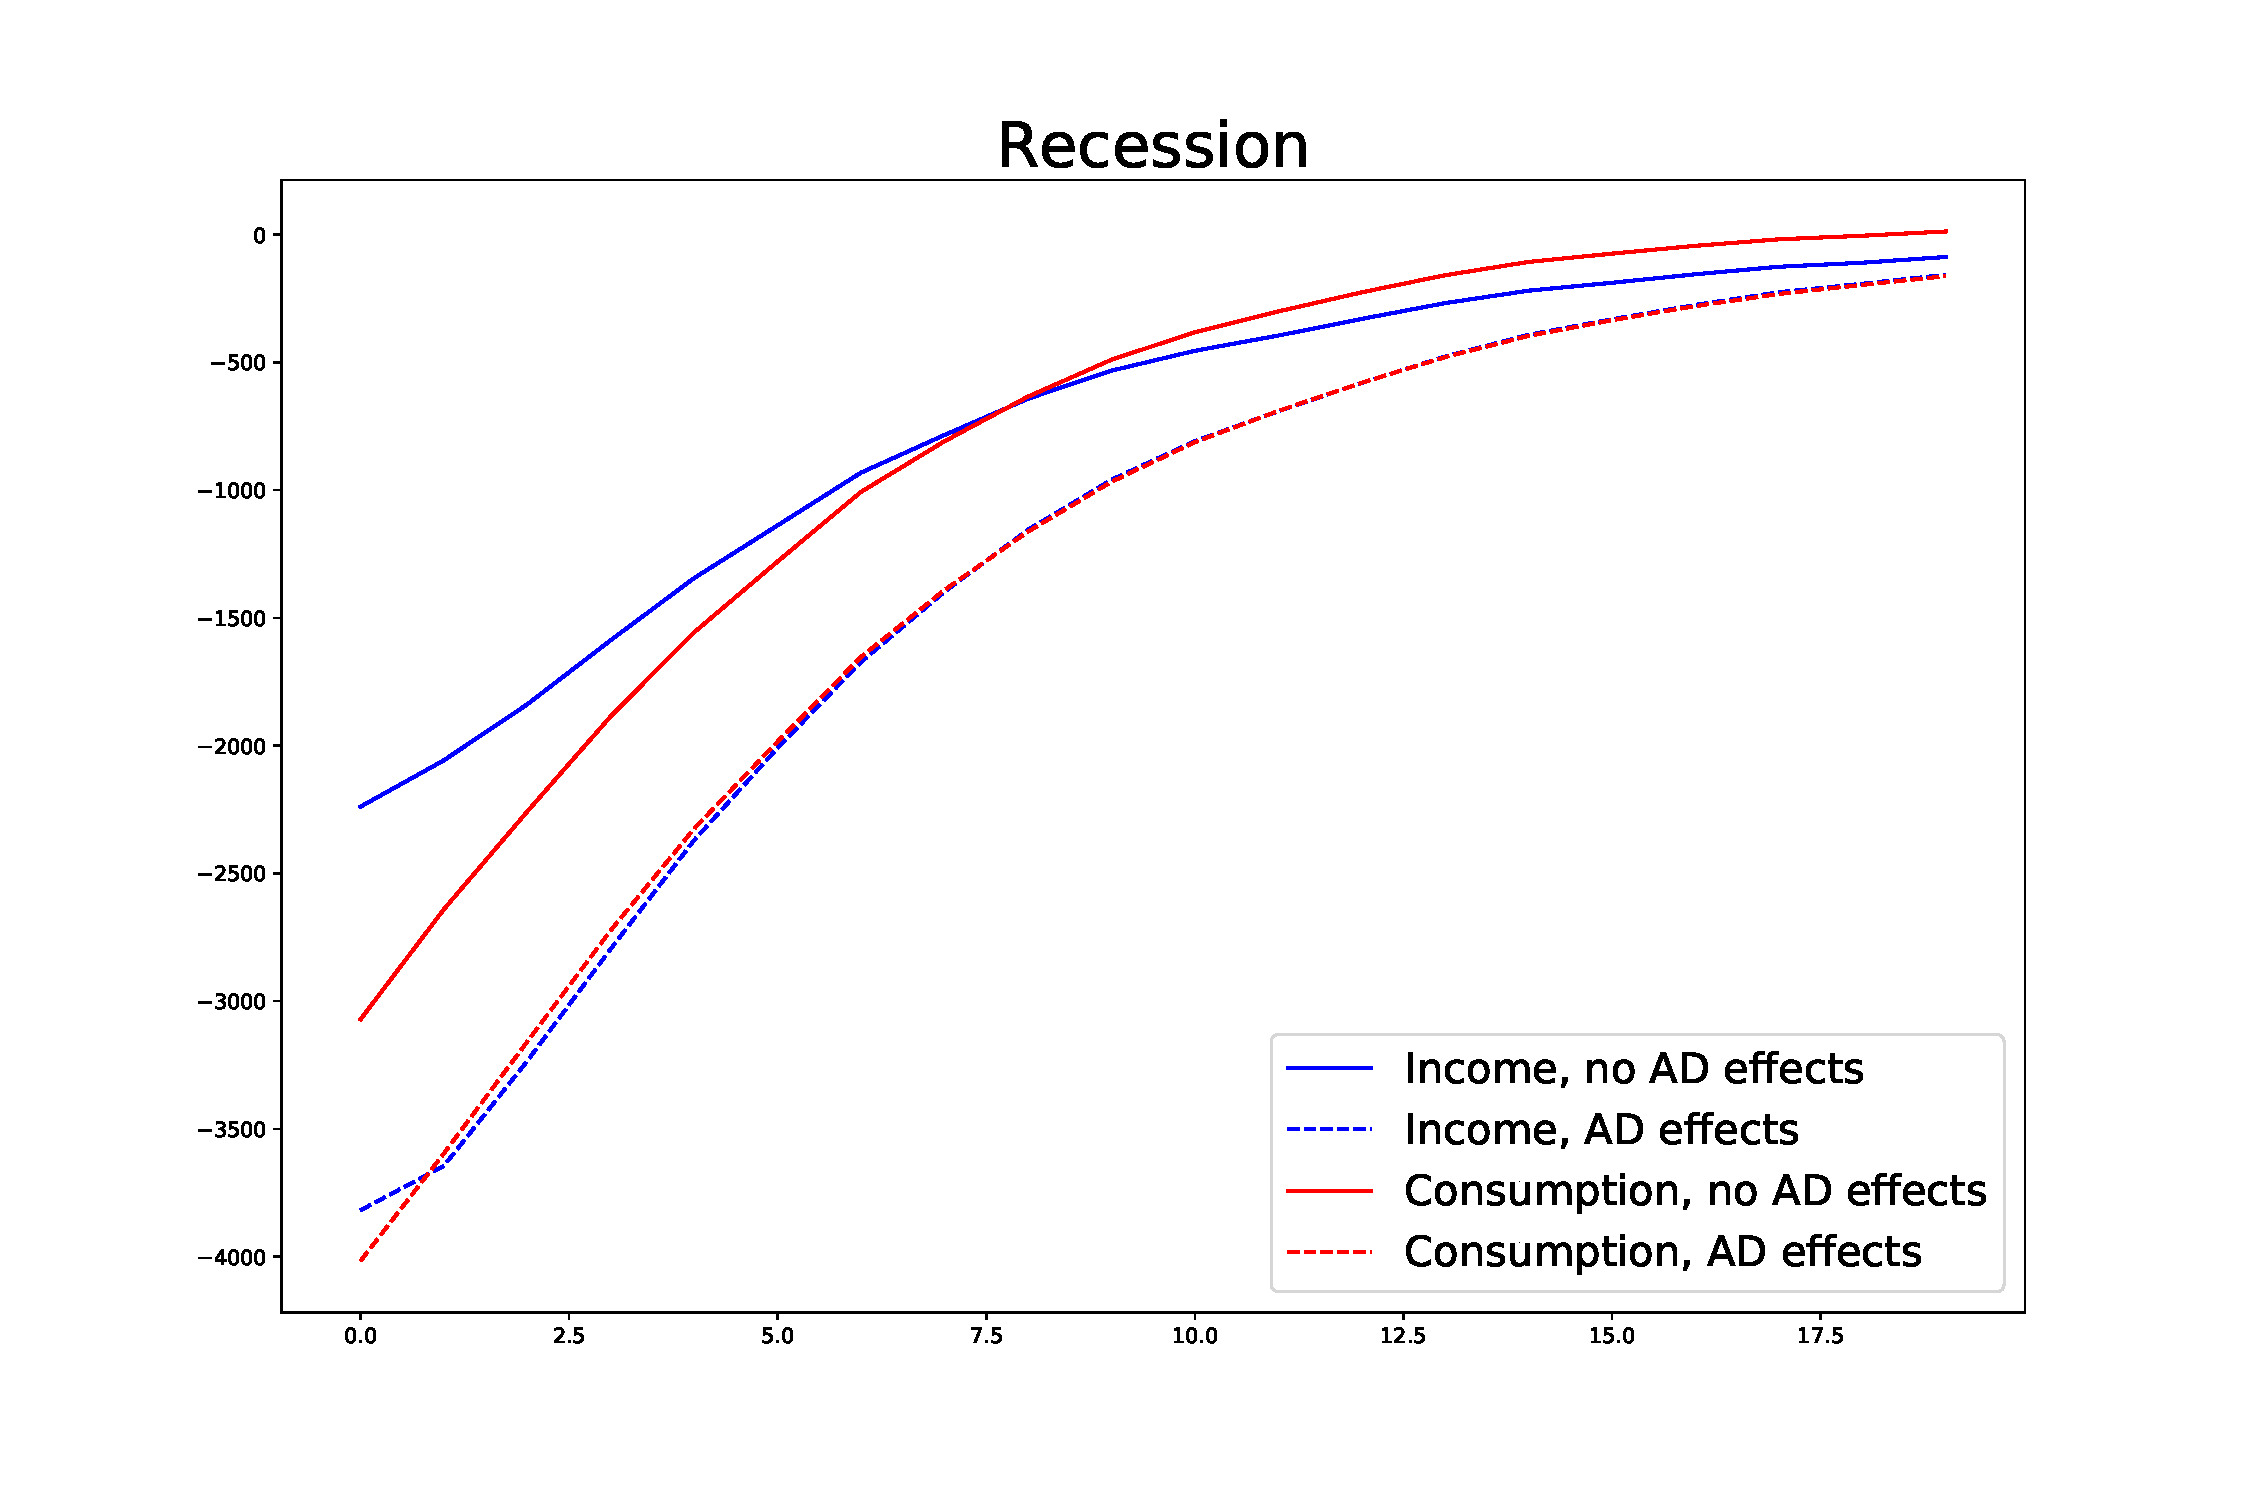
\includegraphics[width=\linewidth]{../50kSample_BaseCal/recession.pdf}
		\caption{Recession}
		\label{fig:recession}
	\end{centering}
\end{figure}

\FloatBarrier
\subsection{Tax cut}

\begin{itemize}
	\item We consider a payroll tax cut by 2 pp for 8q (deterministic length)
	\item See Figure \ref{fig:taxcut}
	\subitem The tax increases income and consequently pushes up consumption
	\subitem The drop in consumption in 9q is due to the fact that the splurge is applied to income in excess of the baseline income, which drops to zero after the tax cut is reversed. Consumption spending remains elevated for some time after the tax cut due to built up savings. 
	\subitem With aggregate demand effects, the effect on consumption is larger as the increased consumption reinforces consumption through higher income due to higher TFP	
\end{itemize}

\begin{figure} 
	\begin{centering}
		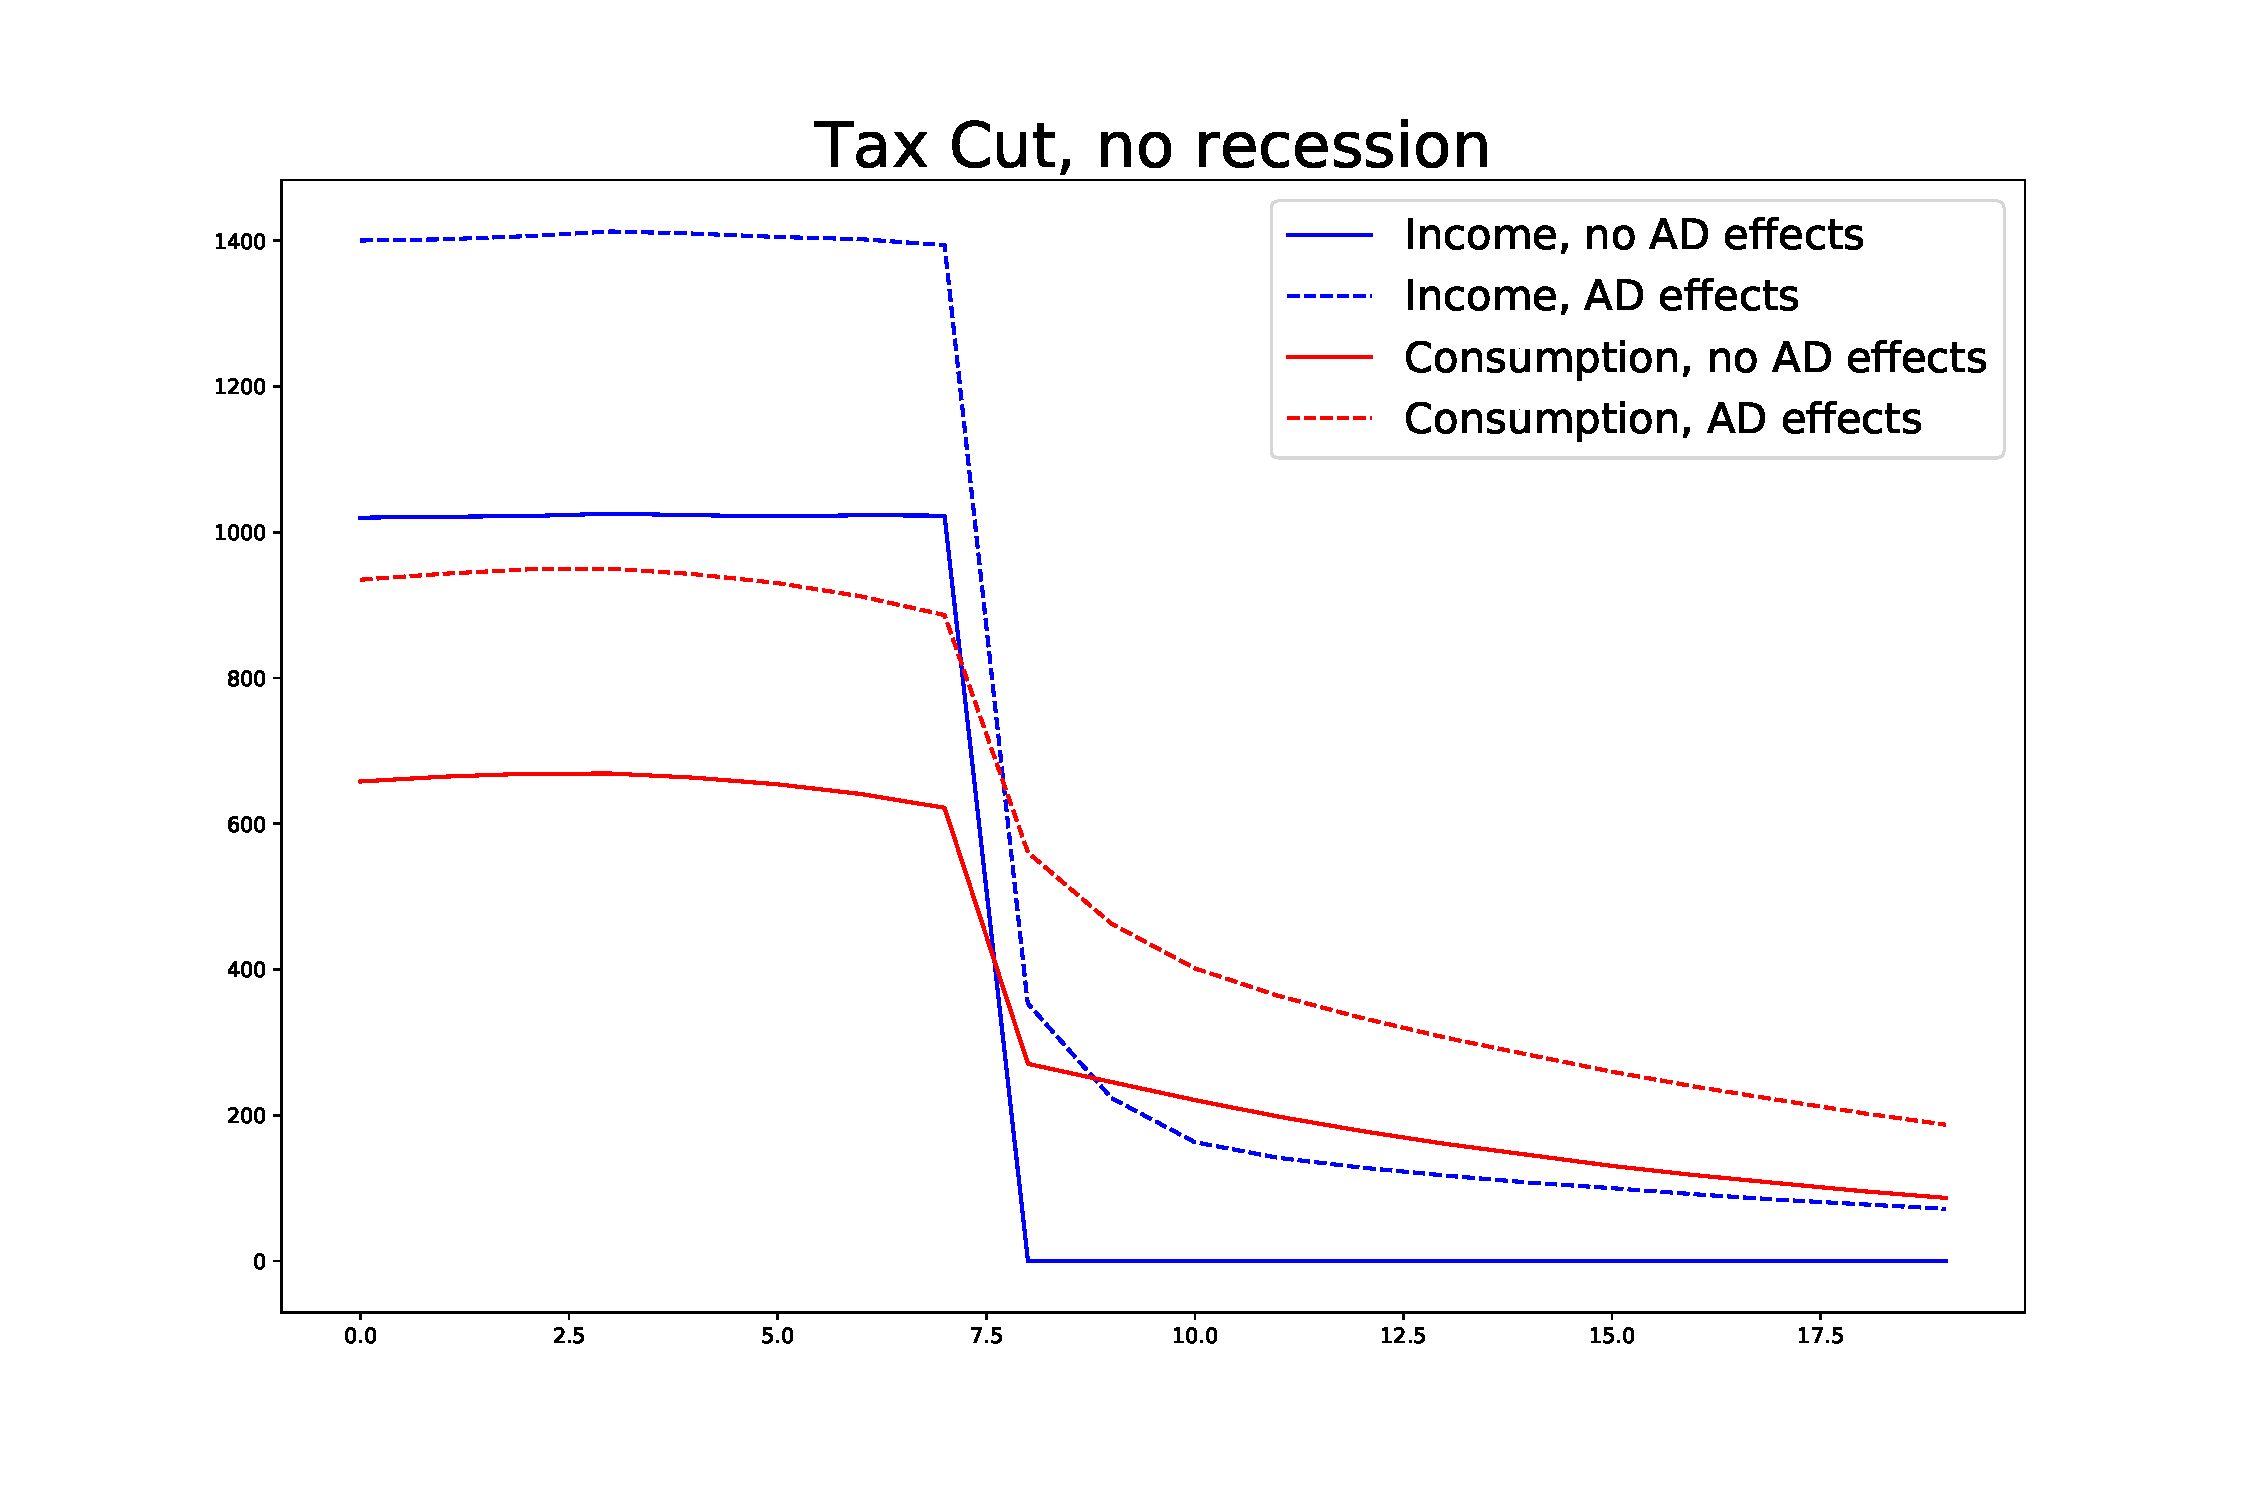
\includegraphics[width=\linewidth]{../50kSample_BaseCal/tax_cut.pdf}
		\caption{Tax cut}
		\label{fig:taxcut}
	\end{centering}
\end{figure}

\FloatBarrier
\subsection{Tax cut during recession}

\begin{itemize}
	\item We consider a payroll tax cut by 2 pp for 8q (deterministic length) during a recession with an expected length of 6q 
	\item Additional income / consumption relative to the baseline (see figure \ref{fig:taxcutrecession}) and to recession scenario (see figure \ref{fig:taxcutrecession2})
	\item When AD effects are switched off we obtain a similar result as in the baseline. However, note, that as the recession disappears, the additional income by the tax cut increases as more people are employed
	\item This upward trend in the effect of the tax cut is much more pronounced when considering AD effects. This is because very low consumption at the beginnning of the recession sets a much steeper recovery path.
	\item Not clear why consumption first drops (numerical error?)
\end{itemize}

\begin{figure} 
	\begin{centering}
		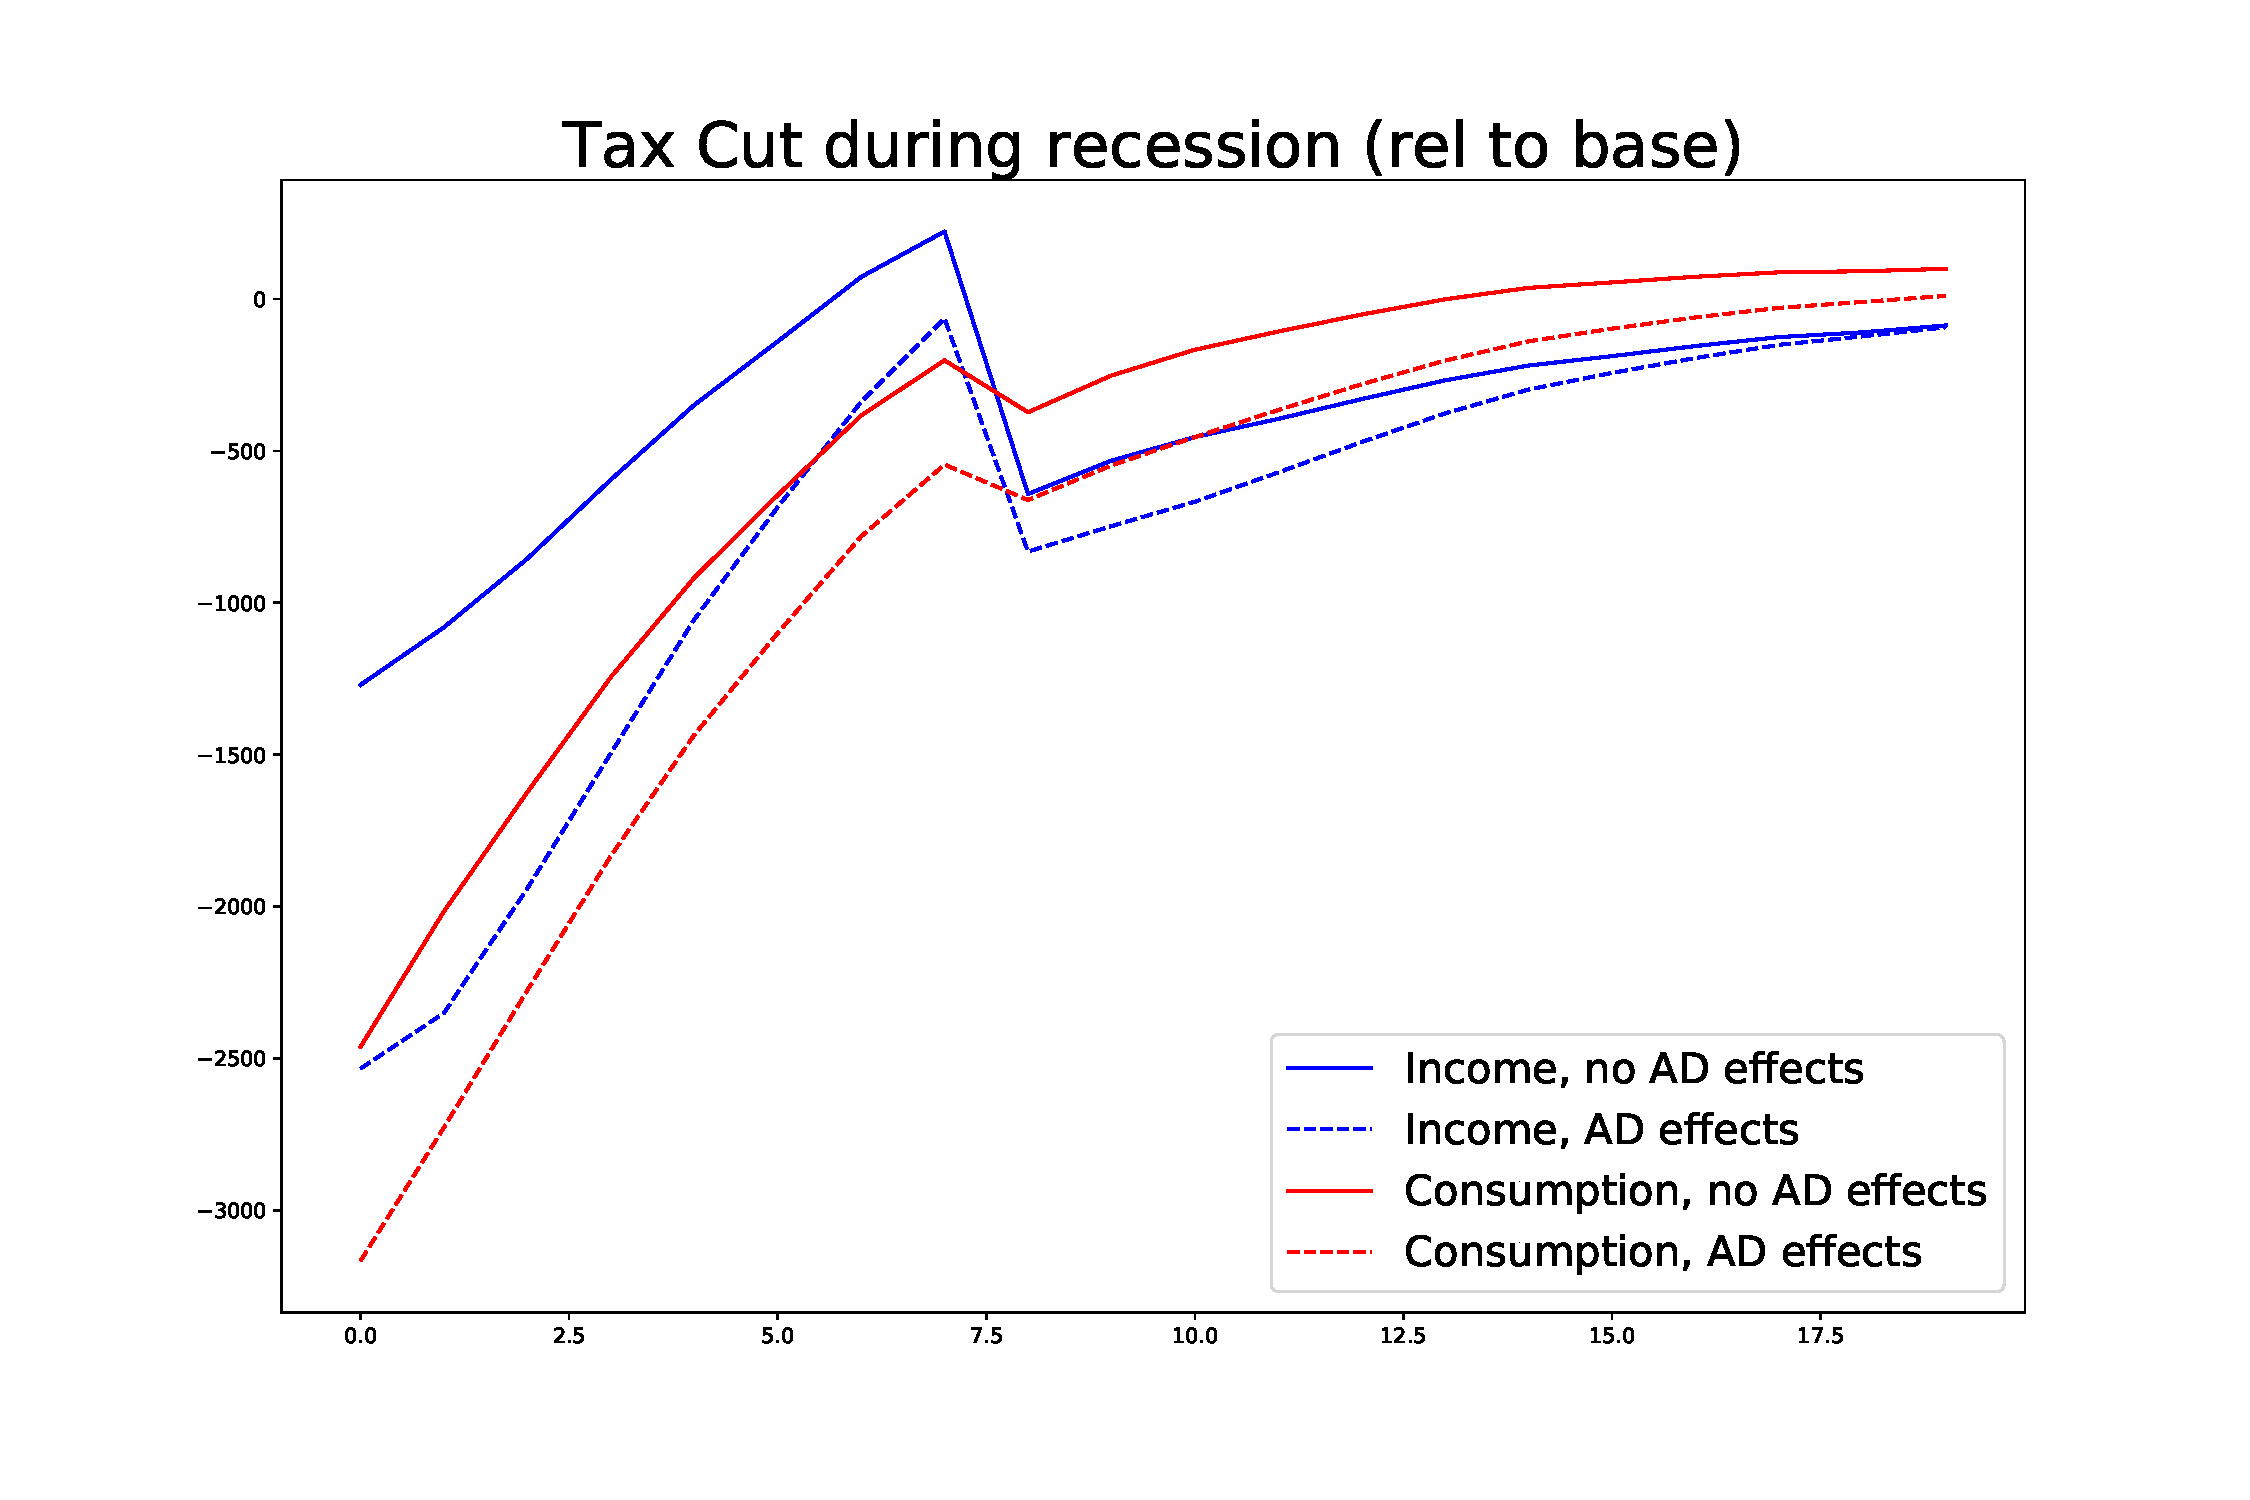
\includegraphics[width=\linewidth]{../50kSample_BaseCal/taxcut_recession.pdf}
		\caption{Tax cut during a recession}
		\label{fig:taxcutrecession}
	\end{centering}
\end{figure}
\begin{figure} 
	\begin{centering}
		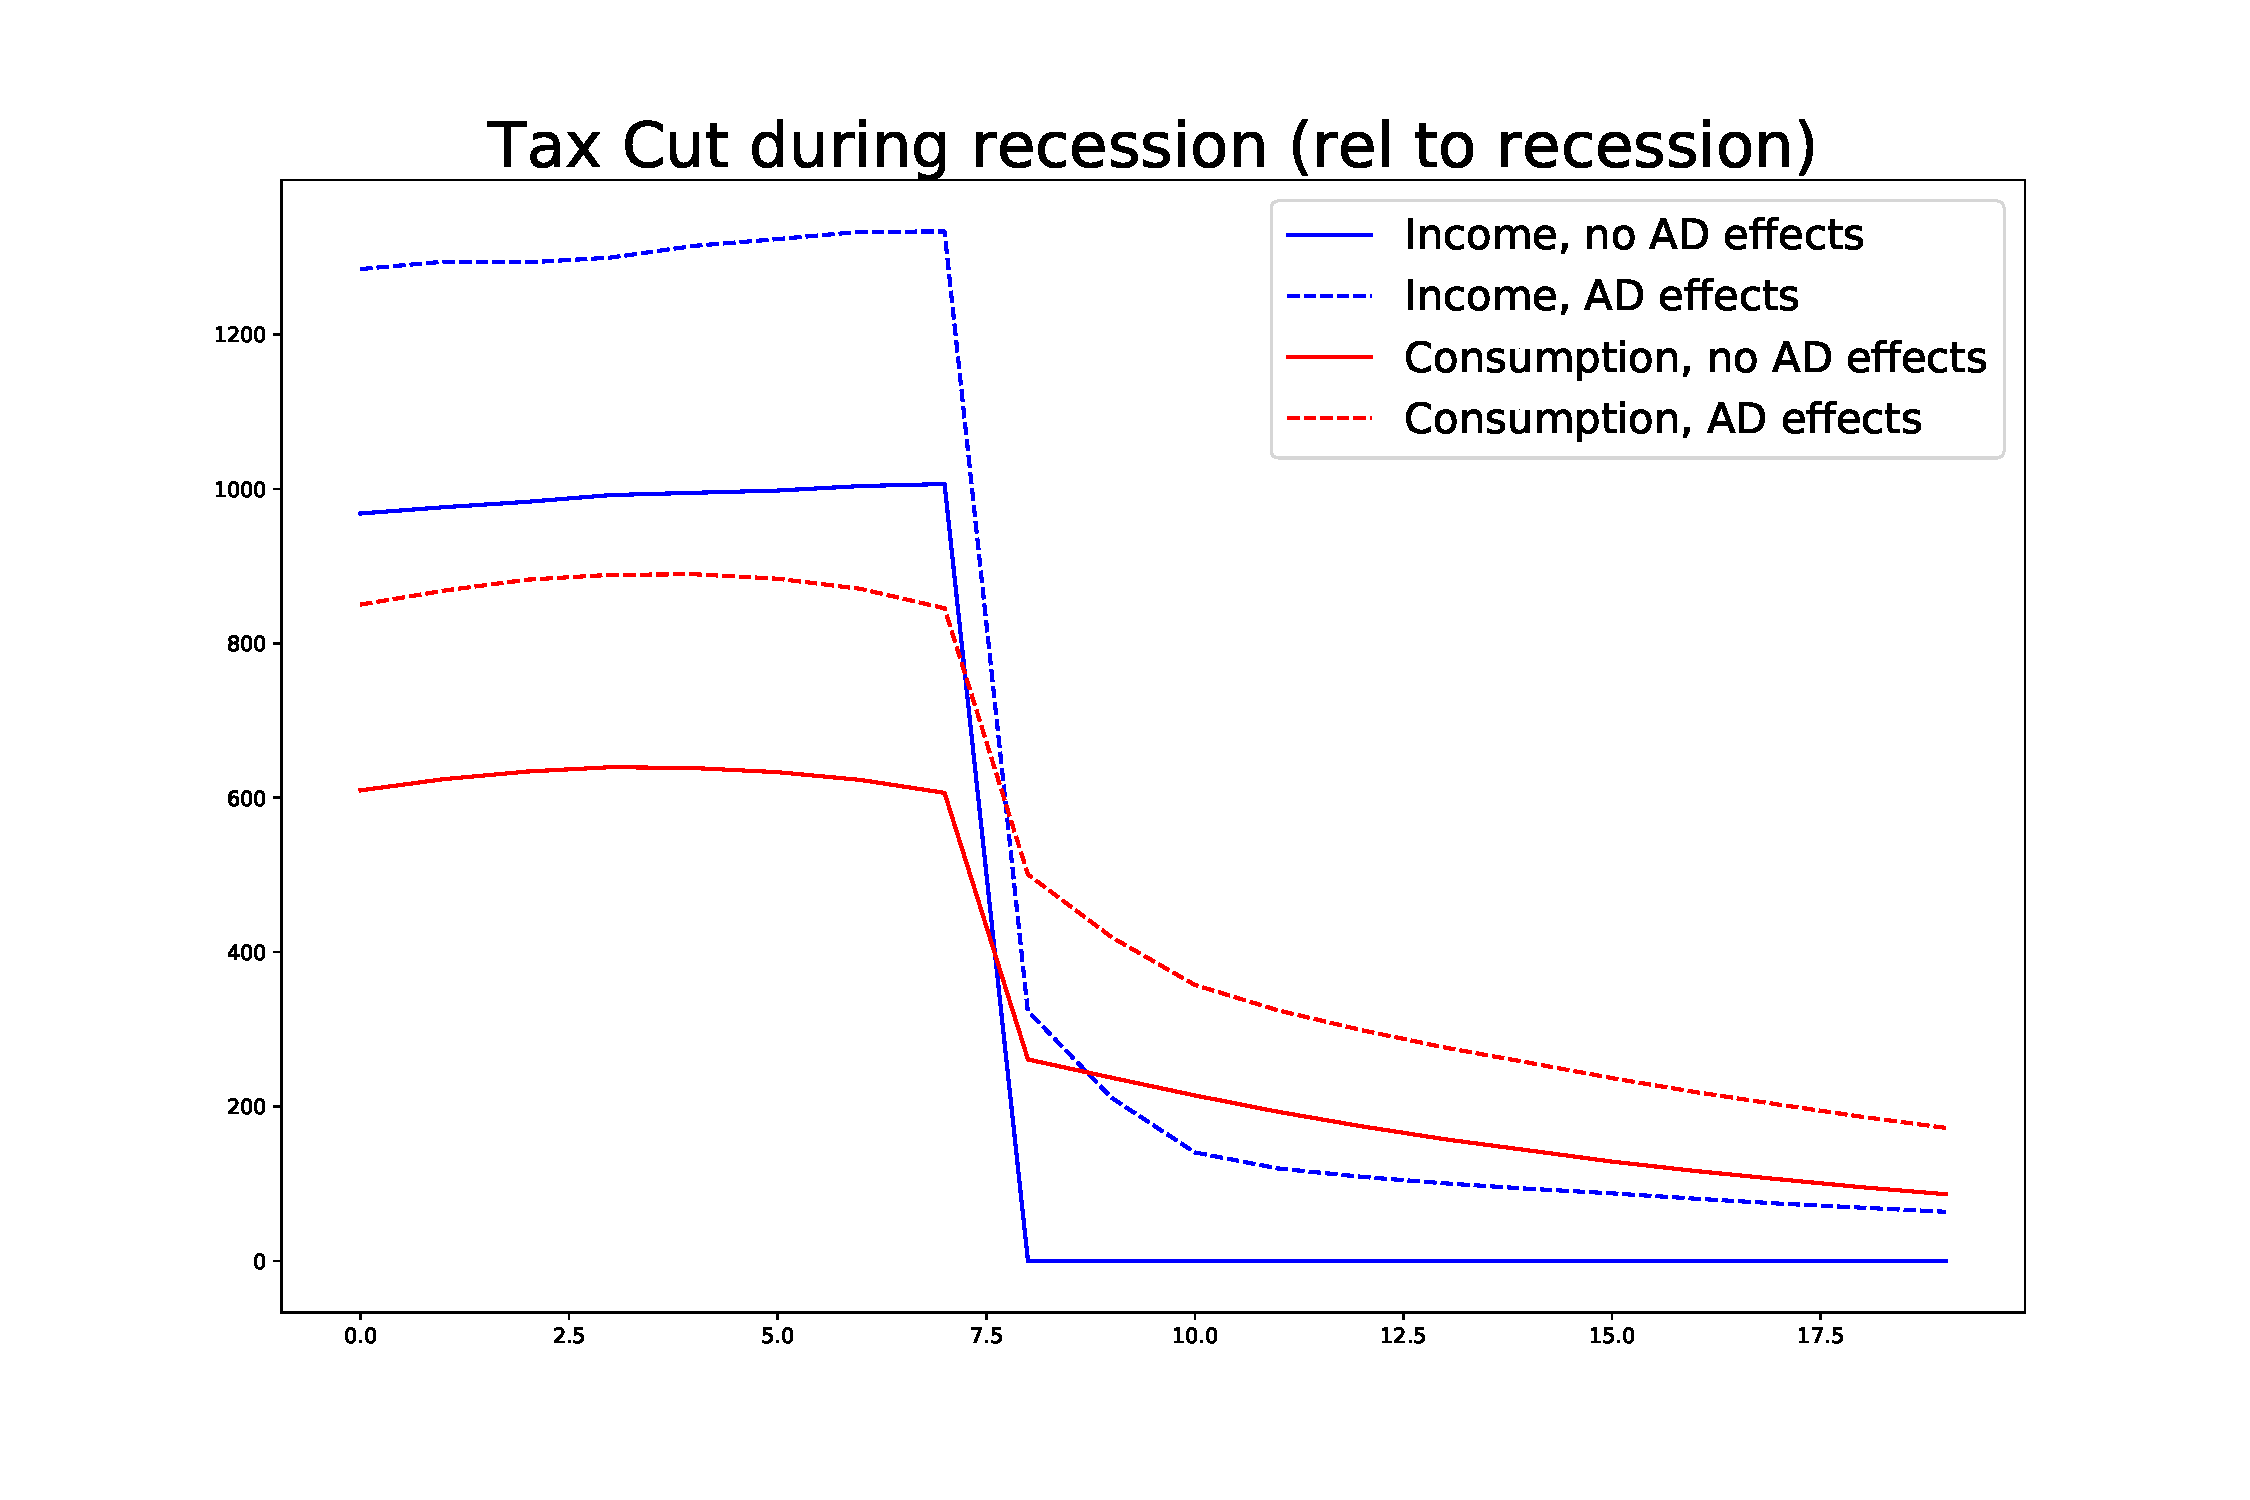
\includegraphics[width=\linewidth]{../50kSample_BaseCal/taxcut_recession2.pdf}
		\caption{Tax cut during a recession}
		\label{fig:taxcutrecession2}
	\end{centering}
\end{figure}

\FloatBarrier
\subsection{[Preliminary] Comparing magnitude of stimulus relative to policy expenditure}

\begin{itemize}
	\item Figure \ref{fig:stimulus} shows the additional consumption caused by the policy relative to the total net present value of the policy intervention
	\item However, we use the net present value from the no AD scenario
	\item This is problematic, need to calculate the amount of additional expenditure due to the fiscal policy intervention -> 2pp x recession-Ad-income
\end{itemize}

\begin{figure} 
	\begin{centering}
		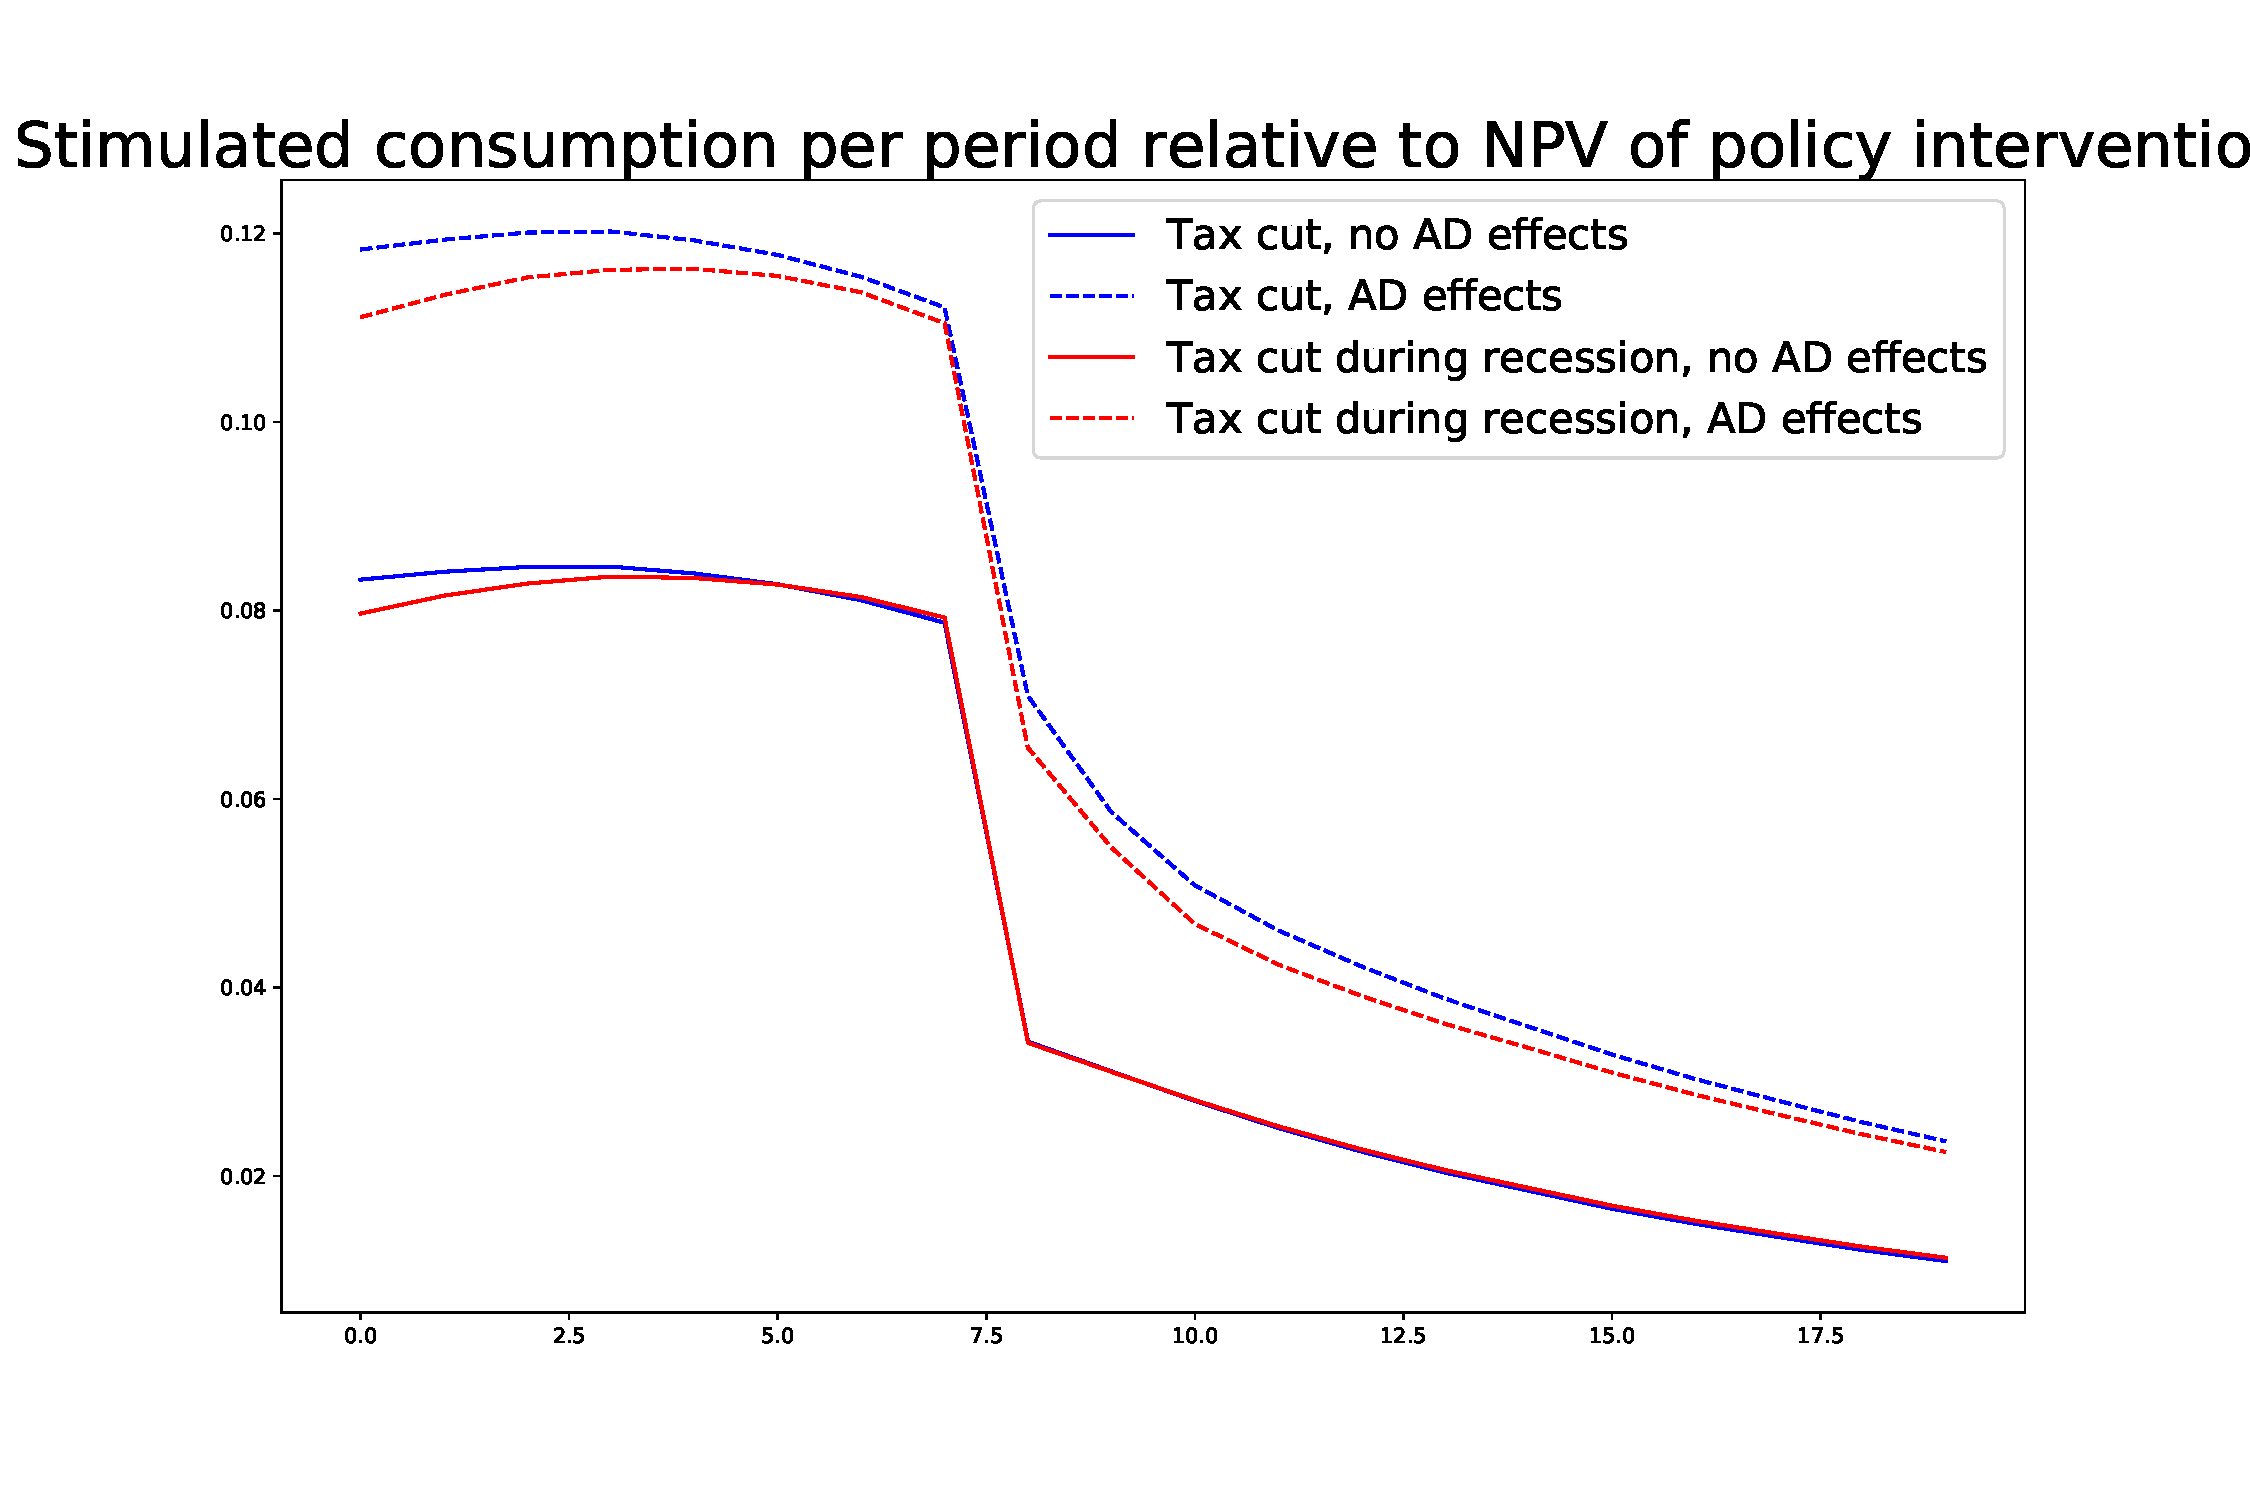
\includegraphics[width=\linewidth]{../50kSample_BaseCal/stimulated-consumption.pdf}
		\caption{Stimulus}
		\label{fig:stimulus}
	\end{centering}
\end{figure}





\end{document}
